\message{ !name(../thesis.tex)}%Input Macros (i.e. write your own macros file called MacroFile1.tex)
%\include{Macros/MacroFile1}

\documentclass[oneside,12pt]{classes/CUEDthesisPSnPDF}

% \ifpdf
%     \pdfinfo { /Title  (Goncalves NR - PhD Thesis)
%                /Creator (TeX)
%                /Producer (pdfTeX)
%                /Author (Nuno Reis Goncalves nrg30@cam.ac.uk)
%                /CreationDate (D:20150101000000)  %format D:YYYYMMDDhhmmss
%                /ModDate (D:20150101000000)
%                /Subject (Imaging Local Circuits In The Human Brain)
%                /Keywords (fMRI, vision, binocular disparity)}
%     \pdfcatalog { /PageMode (/UseOutlines)
%                   /OpenAction (fitbh)  }
% \fi

\title{Neural computation of depth from binocular disparity}

\ifpdf
  \author{\href{mailto:nrg30@cam.ac.uk}{Nuno Goncalves}}
  \collegeordept{\href{http://www.sid.cam.ac.uk}{Sidney Sussex College}}
  \university{\href{http://www.cam.ac.uk}{University of Cambridge}}
  \crest{\includegraphics[width=30mm]{UnivShield}} % insert the file name that contains the crest in-place of 'UnivShield'
\else
  \author{Nuno Goncalves}
  \collegeordept{Sidney Sussex College}
  \collegeordept{Department of Psychology}
  \university{University of Cambridge}
  \crest{\includegraphics[bb = 0 0 292 336, width=30mm]{UnivShield}}
\fi

%\renewcommand{\submittedtext}{change the default text here if needed}
\degree{Doctor of Philosophy}
\degreedate{September 2015}

% turn of those nasty overfull and underfull hboxes
\hbadness=10000
\hfuzz=50pt

% Put all the style files you want in the directory StyleFiles and usepackage like this:
\usepackage{style-files/watermark}

% Comment out the next line to get single spacing
\onehalfspacing

\begin{document}

\message{ !name(introduction/introduction.tex) !offset(-50) }
%%% Thesis Introduction --------------------------------------------------
\chapter{Introduction}
\ifpdf
    \graphicspath{{Introduction/IntroductionFigs/PNG/}{Introduction/IntroductionFigs/PDF/}{Introduction/IntroductionFigs/}}
\else
    \graphicspath{{Introduction/IntroductionFigs/EPS/}{Introduction/IntroductionFigs/}}
\fi

This thesis is about animals with overlapping binocular vision, and particularly about their ability to exctract three-dimensional information from binocular disparity. I will follow a terminology similar to that chosen by David Marr in his book on the computational investigation of vision (Marr's book citation). Specifically, I will use the term \textit{disparity} to describe the angular difference between the projection of a point in three-dimensional space onto the left and right retinae. I will refer to the physical distance between that point and the observer as \textit{distance}. The term \textit{depth} will be used to describe the perceptual experience of distance. In this chapter, I will introduce basic aspects of binocular vision and stereopsis that are necessary to understand the content and relevance of the experimental and theoretical work described in this thesis.  

\section{Binocular vision and stereopsis}
% low priority at the moment 
Perception under binocular viewing is a topic that attracted the attention of many intelectuals throughout the centuries, such as Descartes, Newton, etc (see Rogers and Howard here).

\subsection{Perceptual advantages}
% this is low priority at the moment
% for perceptual advantages see Allman, Evolving brains
For animals with laterally positioned eyes, we find increase in panoramic vision, meaning that these animals can capture visual information over a large portion of the space around them. Mammals typically have a considerable overlap between their monocular fields. What can be the reasons that may outweigh the loss of panoramic vision?
% Would like to make a figure showing monocular/binocular overlap for mammals (mouse, rat, cat, monkey and human) - later if time permits 

Also look at: Ohzawa, what do animals see?

First I will explain what are the advantages of having two (frontally positioned overlapping) eyes (all the earlier reports ... )
Binocular vision (generally, not necessarily related to depth perception)

\begin{enumerate}
\item reading 
\item reaching/grasping 
\item rivalry
\item motion
\end{enumerate}

At the end of this subsection I should point to the idea that having two eyes gives us two images of the world acquired from different points, and that the positional differences between particular features of these images can inform us about the depth structure of the scene. To understand why this happens, we need to look into the geometry of the binocular system. 

\subsection{Basic geometry of binocular vision}\label{sec:basic-geom-binoc}

Our eyes are horizontally separated and, hence, each eye samples the visual world from a different vantage point. As a result, if we assume that an observer maintains constant the position of their eyes, the projections of a three-dimensional object onto the left and right retinae depend on the distance between the object and the observer. To illustrate this, let us consider a point object $P$ in the three-dimensional space (Figure \ref{fig:geostereo}). The observer fixates in a point $F$, which projects to the corresponding points $F_{L}$ and $F_{R}$ in the left and right retinae, respectively. However, the point $P$ projects to non-corresponding points $P_{L}$ and $P_{R}$  in the retinae, depending on the distance between the point $P$ and the observer. Absolute disparity is defined as the difference in angular displacement between the projections of $P$ and $L$. If we denote $\alpha$ and $\beta$ as the angles between the projections of $P$ and $F$ onto the left and right retinae, the absolute disparity is then given by $\delta = \alpha - \beta$.

\begin{figure}
  \centering
  
\includegraphics{absolute-disparity}
  \caption{Basic geometry of stereopsis.}
  \label{fig:geostereo}
\end{figure}

It is thus clear that absolute disparity depends on the position of $P$. However, it is important to notice that absolute disparity is also a function of the position of $F$ - that is, absolute disparity depends on vergence. Therefore, absolute disparity alone cannot be used to recover the absolute distance between the point object and the observer. Absolute disparity can only tell us about the distance between $P$ and $F$. To know the absolute distance between $P$ and the observer, one needs to know about the position of $F$ in space. Vergence and accommodation signals can be used for this purpose (reference here, see Julesz' book). 
In three-dimensional space, the horopter is a surface defined by all the points that project to corresponding locations in the left and right retinae. Points in the horopter have therefore zero disparity. In the two-dimensional case (i.e. ignoring the vertical dimension), a good approximation to the horopter is the Vieth-M{\"u}ller circle (Figure \ref{fig:dispclass}). In this arrangement, points along the circle are considered to have zero disparity. Non-zero disparities are commonly classified as crossed or uncrossed. Crossed disparities are associated with a temporal shift in relation to the fixation point (compare the projection of $C$ and $F$). Conversely, uncrossed disparities refer to nasal displacements in relation to the fixation point (compare $U$ and $F$). Objects with crossed disparity are therefore closer to the observer in relation to the fixation point, while objects with uncrossed disparity are further away. Although the terms crossed and uncrossed disparity are usually used to denote the disparity produced by near and far objects, it is worth noting that it is not always the case that objects closer to the observer produce crossed disparities, nor that objects further away always produce uncrossed disparities. Strictly, the disparity associated to an object within the Vieth-M{\"u}ller circle is termed convergent disparity, while the disparity produced by an object outside the Vieth-M{\"u}ller circle is called divergent disparity (Howard and Rogers citation).

\begin{figure}
  \centering
  \includegraphics{disparity-classification}
  \caption{Disparity classification and the Vieth-M{\"u}ller circle. Adapted from Howard and Rogers.}
  \label{fig:dispclass}
\end{figure}

Based on figure \ref{fig:dispclass}, we can also introduce the concept of relative disparity between any two points. The relative disparity between $C$ and $U$ is simply defined as the difference between their absolute disparities, $\delta_{CU} = \delta_{C} - \delta_{U}$. Since $\delta  = \alpha - \beta$ (Figure \ref{fig:geostereo}), the expression for relative disparity can be written as $\delta_{CU} = (\alpha_C-\alpha_U) - (\beta_C-\beta_U)$. Here, the absolute distance to the fixation point $F$ is no longer determinant in the measure of disparity.

So far, we have only considered point objects located in the gaze plane (i.e. the transverse plane that divides the retina in superior and inferior portions), which can only produce disparities along the horizontal axis. However, the image projections of a point located elsewhere may be vertically displaced - these displacements are known as vertical disparities. Whether or not vertical disparities occur first depends on the coordinate frame in which disparities are measured. For instance, under the Helmholtz optic array formulation no real point object can create a vertical disparity and, therefore, vertical disparities are necessarily non-epipolar (Erkelens \& van Ee, 1998, Howard and Rogers,2002; \cite{Read2009}). In retino-centric coordinates, the projections of point objects onto the left and right retinae can be vertically displaced (Figure \ref{fig:vertdisp}, adapted from \cite{Read2009}). The vertical displacement itself also varies depending on how elevation is mapped onto a vertical coordinate on the retina (Figure \ref{fig:vertdisp}, compare longitude and latitude mapping). Read and colleagues \cite{Read2009} have analytically demonstrated that retinal vertical disparities vary with viewing conditions depending on the initial geometrical formalization of this problem.

\begin{figure}
  \centering
  \includegraphics{vertical-disparities}
  \caption{Vertical disparities on elevation-longitude and elevation-latitude coordinate frames. Adapted from \cite{Read2009}.}
  \label{fig:vertdisp}
\end{figure}

In this section, I have explained that the horizontal separation of the eyes causes the projection of a given point in space to fall in different positions in the left and right retinae. The displacement between the left and right projection is called a binocular disparity. Binocular disparity varies as a function of the position in the three-dimensional space, and therefore this information can be used to estimate depth in a visual scene. In the next section, I will introduce the behavioural investigations which proved that humans and other mammals make use of this cue for perceiving depth.

% this section needs polishing and much more attention to references. 

\subsection{Stereoscopic depth perception}

We have previously seen how the horizontal separation of the eyes gives rise to binocular disparities. It has long been known that humans explore binocular disparity as a cue to depth, when Wheatstone reported that if the two-dimensional perspective views as seen from each eye of a solid object were presented separately to each eye, observers perceive the three-dimensional configuration of that object (\cite{Wheatstone:1838xf}). Whether binocular disparity alone could support depth perception was unknown, because Wheatstone's experiments lacked obviation of non-visual cues, such as vergence and accommodation. In fact, Donders defended that eye movements were necessary in order to use binocular disparity as a cue to depth perception (\cite{Donders1867}, double-check this reference). However, Heinrich Dove had reported that stereopsis occurred for images that were displayed for a very brief period of time - the time of an electric spark, approximated by less that 1 millisecond - before any eye movements could occur (\cite{Dove1841,Dove1860}), demonstrating that humans do not need vergence and accommodation cues to extract depth information from binocular disparity. 

(now Julezs and the random-dot-stereogram).

Depth in correlated and anti-correlated stereograms.

% Wheatstone, disparity is necessary for stereopsis
% Dove, disparity is sufficient for stereopsis

% should I talk briefly about vergence and accommodation here?

In the introduction to the geometry of binocular vision (\ref{sec:basic-geom-binoc}), we defined two different types of binocular disparity - absolute and relative binocular disparity, which can both be used to estimate depth. However, humans are able to explore relative disparities to a much greater extent when compared to absolute disparities (...)   

We have also seen that vertical disparities can occur during natural viewing (\ref{fig:vertdisp}). But are humans able to use this information for depth perception? 
Depth from vertical disparity (Rogers and Bradshaw, etc.).
Tolerance to vertical disparities.

The experimental evidence introduced here highlights the exquisite sophistication of the visual system, and that binocular disparity is a powerful cue used by humans to estimate depth. These remarkable findings led researchers to investigate the neurophysiological mechanisms underlying this ability.

\section{Neural encoding of binocular disparity}  % focus on descriptive view
% it is important to mention the pathways up to V1/V2 very well, including laminar investigations of binocularity and feed forward/feedback connections. From V2 upwards we need to spend a lot of time on MT and IT because of the monkeys, and then talk about various areas that light up based on fMRI

\subsection{Binocularity along the visual pathways}
% this subsection should be brief here, it's just to help framing the next two paragraphs
Start with Hubel and Wiesel, Poggio, etc... Here the point is to highlight when binocular processing is likely to take place (rate stim in 2 eyes > rate stim in 1 eye) 

The information captured by each eye is relayed to the LGN and then fed to layer 4C of primary visual cortex. Neurons along this pathway are primarily driven by monocular stimulation, although modulations depending on binocular information may be observed in the LGN (ref). That is, one can only map the area of the input space that causes neurons to fire in one of the eyes. Therefore, such cells are called monocular neurons. Given that monocular neurons do not seem to be driven by inputs in one of the eyes, these cells do not seem capable of encoding binocular disparity. Instead, the first steps of binocular processing are likely to take place in extra-granular layers of V1, where receptive fields in both eyes can be mapped for many neurons - these are called binocular cells (need facts and figures here).

V2... etc..
Should put more emphasis on visual pathways, laminar organization, feedback and feed-forward connections...

\subsection{Disparity selectivity}
Here I will start with Barlow and go all the way to Poggio.
The idea here is to show disparity selectivity in terms of physiology (i.e. tuning properties of disparity selective neurons across the cortex)
I will start with V1 and then will go into V2, MT, IT (emphasize the stereo correspondence problem)

Look at Smolyanskaya 2015 Neuron

\subsection{Joint encoding of motion cues to depth}

\section{Computation of depth from binocular disparity} % focus on mechanistic view

So far, I have briefly introduced the geometry of human binocular vision and I have reviewed evidence that humans can extract precise depth information from binocular disparity in isolation. The last section was devoted to showing that many neurons across the neocortex are selective to depth from binocular disparity. In this final section of the introduction, my aim is to review the computational theories of stereopsis that aim to relate behavior and neurophysiological evidence.

\subsection{Marrian analyses: computation that needs to be done}
Three levels of computation (purpose, algorithmic, hardware..., right?)

\subsection{Disparity energy model}

Ohzawa and colleagues propose a model that shaped the following two decades of investigations on stereopsis \cite{Ohzawa:1990cq}. 

\section{Thesis Overview} 
% here I will outline how this work will try to advance our understanding of binocular vision as outlined above.

%%% ----------------------------------------------------------------------


%%% Local Variables: 
%%% mode: latex
%%% TeX-master: "../thesis"
%%% End: 

\message{ !name(../thesis.tex) !offset(-82) }

\end{document}
